\documentclass[11pt,onecolumn]{IEEEtran}

\usepackage{amsmath,amssymb}
\usepackage{booktabs}
\usepackage{graphicx}
\usepackage{xurl}
\usepackage{placeins}

\graphicspath{{../figures/}}
\emergencystretch=2em

\title{Supplementary Material for ``Projection-Selected Multidimensional Candan Refinement after FFT Tensor Support Selection''}
\author{Yuhui Liu and Hangcheng Han}

\begin{document}
\maketitle

The main manuscript presents the complete method and primary evidence. This supplementary material supports deeper inspection through expanded local-family ledgers, executable definitions, full-offset results, physical-parameter accuracy, quotient-stability evidence, controlled near--far metrics, and independent MATLAB replication.

\section{Reproducibility Map}

The controlled local-family campaign is reproduced by
\path{04_experiments/eval/run_tsp_controlled_local_family_baselines.py}; its
1200 common test scenes, 480 disjoint validation scenes, row-level timings,
and work contracts are stored in
\path{05_results/tsp_controlled_local_family_paper}. Unified steady-state timing is reproduced by
\path{run_tsp_unified_runtime_benchmark.py} and stored in
\path{05_results/tsp_unified_runtime_paper}. Full-offset results are reproduced by
\path{run_tsp_full_offset_sweep.py}. The controlled separation and
near--far campaign is reproduced by
\path{run_tsp_candan_stress_zeta_audit.py}. The projection protocol and runtime
audits are reproduced by \path{run_tsp_candan_gate_protocol_audit.py} and
\path{run_tsp_projection_gate_runtime.py}. The 9000-scene physical and $\zeta$
replay is reproduced by \path{run_tsp_candan_physical_zeta_audit.py}. Their
registered result directories contain commands, configurations, seeds,
environments, manifests, and row-level ledgers.

The independent MATLAB package in \path{04_experiments/matlab} implements the
synthetic geometry with portable scene seeds. In particular,
\path{exp6_candan_independent_audit.m} is the separate 1200-scene replication
of the complex three-sample update. Run manifests store commands,
configurations, seeds, environments, and metrics beside each output directory.
All manuscript and supplementary figures are generated by
\path{manuscript_tsp_2026/matlab_figures/generate_tsp_figures.m}; the source
reads the registered CSV artifacts and exports vector PDF/SVG plus
300/600-dpi raster companions.

\section{Controlled Local-Family and Broader Comparisons}

\begin{table*}[!ht]
\centering
\caption{Controlled local-family results on 1200 common test scenes. Intervals are Student-$t$ 95\% intervals over five seed means. Improved denotes the fraction of scenes whose clean-channel NMSE is lower than that of the grid estimate.}
\label{tab:supp_local_family}
\scriptsize
\setlength{\tabcolsep}{3.0pt}
\begin{tabular}{lcccc}
\toprule
Method & NMSE [95\%] (dB) & Gain (dB) & Half-bin [95\%] & Improved \\
\midrule
Grid FFT top-$L$ & $-5.43\,[-5.53,-5.33]$ & 0.00 & $71.9\,[69.7,74.1]\%$ & -- \\
Quadratic power three-sample & $-6.04\,[-6.13,-5.94]$ & 0.61 & $71.9\,[69.7,74.2]\%$ & 100.0\% \\
Candan complex three-sample & $-29.69\,[-30.33,-29.05]$ & 24.26 & $79.6\,[77.9,81.3]\%$ & 100.0\% \\
One-step fixed-support Newton & $-7.71\,[-7.85,-7.58]$ & 2.28 & $71.7\,[69.4,74.0]\%$ & 99.4\% \\
Cartesian local & $-12.73\,[-12.81,-12.65]$ & 7.30 & $79.6\,[77.9,81.3]\%$ & 100.0\% \\
\bottomrule
\end{tabular}
\end{table*}


All local-family methods share each noisy tensor, known $L$, the FFT top-$L$
support, periodic coordinates, and joint-LS convention. Unified runtime results
are reported separately in Table~\ref{tab:supp_projection_runtime} to avoid
mixing the common local-family ledger with the dedicated projection-selection
implementation. In that audit, Candan takes 11.07 ms and projection-selected
Candan takes 11.24 ms. The grid fitted energy is the sum of selected FFT-bin
energies, so no second LS solve is required.

\begin{table}[!ht]
\centering
\footnotesize
\caption{Unified 1200-scene runtime audit (one thread, complex128, median of three repetitions).}
\label{tab:supp_projection_runtime}
\begin{tabular}{lrrr}
\toprule
Method & Update (ms) & Decision (ms) & End to end (ms) \\
\midrule
Candan & 1.92 & 0.00 & 11.07 \\
Explicit two-residual implementation & 1.92 & 0.70 & 18.98 \\
Projection-selected Candan & 1.93 & 0.14 & 11.24 \\
\bottomrule
\end{tabular}
\end{table}


\begin{table}[!ht]
\centering
\caption{Broader matched accuracy endpoints on the same 1200-scene tensor set.}
\label{tab:supp_broader}
\footnotesize
\begin{tabular}{lrrl}
\toprule
Method & NMSE (dB) & Half-bin & Role \\
\midrule
Grid FFT top-$L$ + LS & $-5.43$ & 0.719 & support baseline \\
Candan complex three-sample + LS & $-29.69$ & 0.796 & matched interpolation \\
Cartesian local + LS & $-12.73$ & 0.796 & fixed support \\
Complex PARAFAC-ALS & $-16.85$ & 0.524 & factor reconstruction \\
NOMP-inspired & $-53.39$ & 0.999 & iterative continuous \\
\bottomrule
\end{tabular}
\end{table}

\section{Executable Local-Baseline Definitions}

Let $X[\mathbf{k}]=\operatorname{FFTN}(\mathcal{Y})[\mathbf{k}]$,
$P[\mathbf{k}]=|X[\mathbf{k}]|^2$, and
let $\mathbf{k}_\ell$ be a selected top-$L$ bin. For axis $d$, the
quadratic power three-sample route holds every other coordinate at $\mathbf{k}_\ell$ and uses
\begin{equation}
 \widehat{\delta}_{d,\ell}
 =\operatorname{clip}_{[-1/2,1/2]}
 \frac{P[\mathbf{k}_\ell-\mathbf{e}_d]
       -P[\mathbf{k}_\ell+\mathbf{e}_d]}
 {2\{P[\mathbf{k}_\ell-\mathbf{e}_d]
       -2P[\mathbf{k}_\ell]
       +P[\mathbf{k}_\ell+\mathbf{e}_d]\}}.
 \label{eq:supp_three_sample}
\end{equation}
Periodic indexing is used. A nonnegative or numerically flat curvature
returns zero offset. After all $DL$ offsets are formed, one joint LS fit uses
the interpolated coordinates.

The proposed Candan coordinate update applies the finite-length-corrected
complex three-sample ratio independently on each axis:
\begin{equation}
 \widehat{\delta}^{\rm Can}_{d,\ell}
 =\operatorname{clip}_{[-1/2,1/2]}
 \frac{\tan(\pi/N_d)}{\pi/N_d}
 \operatorname{Re}\!\left\{
 \frac{X[\mathbf{k}_\ell-\mathbf e_d]-X[\mathbf{k}_\ell+\mathbf e_d]}
 {2X[\mathbf{k}_\ell]-X[\mathbf{k}_\ell-\mathbf e_d]-X[\mathbf{k}_\ell+\mathbf e_d]}
 \right\}.
 \label{eq:supp_candan}
\end{equation}
It uses periodic indexing, the same selected neighborhoods, and one final
joint LS fit. Equation~\eqref{eq:supp_three_sample} is therefore the executed
quadratic power comparator, not a proxy name for Quinn or Candan.

For the one-step fixed-support Newton comparator, define
$f_\ell(\mathbf{b})=|\mathbf{a}(\mathbf{b})^H\mathbf{y}|^2$ and evaluate its
analytic gradient $\mathbf{g}_\ell$ and Hessian $\mathbf{H}_\ell$ once at
$\mathbf{k}_\ell$. The direction is
\begin{equation}
 \mathbf{p}_\ell=-\mathbf{H}_\ell^\dagger\mathbf{g}_\ell,\qquad
 \mathbf{p}_\ell\leftarrow
 \mathbf{p}_\ell\min\!\left\{1,\frac{0.45}{\|\mathbf{p}_\ell\|_\infty}\right\}.
 \label{eq:supp_newton}
\end{equation}
The first score-improving point among
$\mathbf{k}_\ell+2^{-j}\mathbf{p}_\ell$, $j=0,\ldots,4$, is accepted;
otherwise the coarse bin is retained. Support identities remain fixed, and
one joint LS fit follows the $L$ updates.

The Cartesian route uses
$\mathcal{G}_{0.45}=\{-0.45,-0.225,0,0.225,0.45\}^D$ and selects
\begin{equation}
 \widehat{\mathbf{u}}_\ell
 =\arg\max_{\mathbf{u}\in\mathcal{G}_{0.45}}
 |\mathbf{a}(\mathbf{k}_\ell+\mathbf{u})^H\mathbf{y}|^2.
\end{equation}
Separable contraction evaluates all $5^D L$ scores, followed by local joint
LS. The Cartesian comparator also computes the grid joint-LS residual and
returns the local result when $\rho_0-\rho_1\geq\tau_\rho$.

\section{Full-Offset Candan Evaluation}

\begin{table}[!ht]
\centering
\caption{Full-offset test on 1200 scenes with fractional coordinates in $[-0.49,0.49]$.}
\label{tab:supp_full_offset}
\footnotesize
\begin{tabular}{lrrr}
\toprule
Method & NMSE (dB) & Gain (dB) & Per-component hit (\%) \\
\midrule
Grid FFT top-$L$ & -3.60 & 0.00 & 52.0 \\
Quadratic power three-sample & -5.03 & 1.43 & 58.2 \\
Candan complex three-sample & -18.05 & 14.45 & 65.2 \\
One-step fixed-support Newton & -4.24 & 0.64 & 52.1 \\
Cartesian local & -10.22 & 6.62 & 65.3 \\
\bottomrule
\end{tabular}
\end{table}


The full-offset campaign evaluates 1200 test scenes over
$[-0.49,0.49]$ bin per axis. The row-level bundle records the Candan coordinate
updates, joint-LS reconstruction, per-component assignment, and five-seed
accuracy intervals on the same generated scenes.

\begin{table}[!ht]
\centering
\caption{Candan complex three-sample comparator on the frozen 9000-scene CDL test geometry. Intervals use five seed means.}
\label{tab:supp_candan_cdl}
\footnotesize
\begin{tabular}{crrrr}
\toprule
Profile & Scenes & Grid NMSE & Candan NMSE & Gain [95\%] \\
 & & (dB) & (dB) & (dB) \\
\midrule
CDL-A & 3000 & -9.65 & -19.87 & $10.22\,[10.05,10.40]$ \\
CDL-C & 3000 & -9.97 & -14.88 & $4.91\,[4.58,5.23]$ \\
CDL-D & 3000 & -18.29 & -18.57 & $0.28\,[0.02,0.55]$ \\
\bottomrule
\end{tabular}
\end{table}


\section{Calibration-Free Projection Audit}

The proposed rule uses the analytical decision point $\tau_\rho=0$. Across 60
identity scenes, explicit residual and projection-energy decisions agree within
$5.44\times10^{-15}$; QR and reconstruction-based normalized projection
energies agree within $1.09\times10^{-14}$. On 9000 CDL tests, the rule returns
Candan in 82.0\% of scenes, retains 92.9\% of beneficial updates, and filters
75.7\% of harmful updates.

\begin{table}[!t]
\centering
\caption{Gain relative to grid for calibration-free projection selection on five CDL test seeds. Intervals are paired over seed means.}
\label{tab:candan_gate_profiles}
\scriptsize
\setlength{\tabcolsep}{2.5pt}
\begin{tabular}{lrrrr}
\toprule
Profile & Candan & Proj.-selected & Increment [95\%] & Return \\
 & (dB) & (dB) & (dB) & (\%) \\
\midrule
CDL-A & 10.223 & 10.220 & $-0.003\,[-0.009,0.002]$ & 99.8 \\
CDL-C & 4.907 & 4.907 & $-0.000\,[-0.033,0.032]$ & 93.9 \\
CDL-D & 0.284 & 0.712 & $0.428\,[0.321,0.536]$ & 52.2 \\
All & 5.138 & 5.280 & $0.141\,[0.097,0.186]$ & 82.0 \\
\bottomrule
\end{tabular}
\end{table}

\begin{table}[!ht]
\centering
\footnotesize
\caption{Calibration-free projection selection. Increments and intervals are paired over five seed means.}
\label{tab:supp_projection_protocol}
\begin{tabular}{lrrrrr}
\toprule
Profile & Candan & Selected & Increment [95\%] & Return & Harmful rejection \\
\midrule
A & 10.223 & 10.220 & $-0.003\,[-0.009,0.002]$ & 99.8 & -- \\
C & 4.907 & 4.907 & $-0.000\,[-0.033,0.032]$ & 93.9 & 86.5 \\
D & 0.284 & 0.712 & $0.428\,[0.321,0.536]$ & 52.2 & 74.9 \\
All & 5.138 & 5.280 & $0.141\,[0.097,0.186]$ & 82.0 & 75.7 \\
\bottomrule
\end{tabular}
\end{table}


\begin{figure}[t]
  \centering
  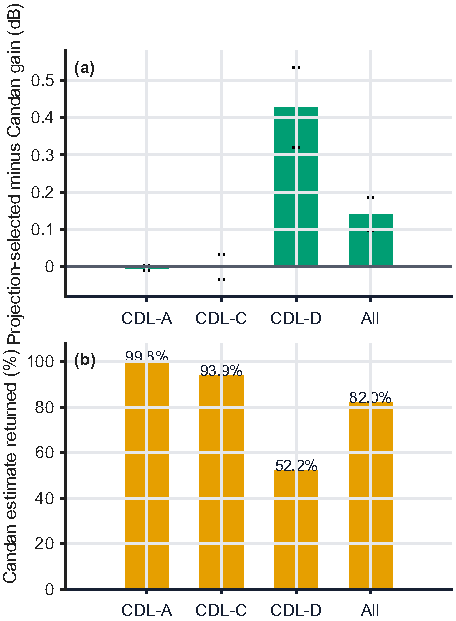
\includegraphics[width=0.62\textwidth]{tsp_candan_gate_profiles.pdf}
  \caption{Profile-level projection behavior on five CDL test seeds. (a) Paired projection-selected-minus-Candan channel-NMSE gain with seed-mean 95\% intervals. (b) Fraction of scenes returning the Candan coordinates under the higher fitted-energy rule.}
  \label{fig:supp_candan_gate_profiles}
\end{figure}

\section{Physical-Parameter and Quotient-Stability Evidence}

\begin{table}[!ht]
\centering
\scriptsize
\caption{CDL physical-parameter results on the same 9000 scenes.}
\label{tab:supp_physical}
\begin{tabular}{lrrrrrr}
\toprule
Profile & \multicolumn{3}{c}{Delay RMSE (ns)} & \multicolumn{3}{c}{Joint quarter-bin hit (\%)} \\
 & Grid & Candan & Selected & Grid & Candan & Selected \\
\midrule
A & 329.74 & 307.77 & 307.76 & 0.8 & 19.5 & 19.5 \\
C & 302.48 & 275.30 & 276.16 & 6.9 & 20.2 & 19.8 \\
D & 653.13 & 659.32 & 656.65 & 14.7 & 17.9 & 17.3 \\
All & 428.45 & 414.13 & 413.52 & 7.5 & 19.2 & 18.8 \\
\bottomrule
\end{tabular}
\end{table}


The physical replay exactly reproduces all 9000 registered channel-NMSE
decisions. Minimum-$\zeta$ percentiles (5th/50th/95th) are 0.015/0.111/0.445
for CDL-A, 0.017/0.165/0.637 for CDL-C, and 0.065/0.305/0.717 for CDL-D.
Across the three profiles, Spearman association
between $\zeta$ and clipping is $-0.525$, $-0.508$, and $-0.506$, respectively,
supporting $\zeta$ as an observable quotient-stability diagnostic.

\section{Derivative and CRLB Sanity Check}

For a complex Gaussian observation with mean
$\boldsymbol{\mu}(\boldsymbol{\eta})$ and covariance $\sigma^2\mathbf I$, the
real-parameter Fisher information used by the implementation is
\begin{equation}
 [\mathbf F(\boldsymbol{\eta})]_{ij}
 =\frac{2}{\sigma^2}\operatorname{Re}\!\left\{
 \left(\frac{\partial\boldsymbol{\mu}}{\partial\eta_i}\right)^H
 \frac{\partial\boldsymbol{\mu}}{\partial\eta_j}\right\}.
\end{equation}
Analytic atom derivatives agree with finite differences to relative error
$5.73\times10^{-10}$. In a separate single-component MATLAB sanity test with
200 trials per SNR, the per-axis RMSE-to-$\sqrt{\mathrm{CRLB}}$ ratio lies in
$[0.98,1.23]$ from 10 to 30 dB, providing an independent derivative and
single-component scale check for the local-refinement implementation.

\FloatBarrier
\section{Controlled Separation and Near--Far Stress}

The stress generator fixes $L=4$, inserts one pair at circular Euclidean
separations $\{0.25,0.5,1,2\}$ bins, cycles the pair axis, and places the other
components at least four bins away. Pair dynamic range is
$\{0,10,20\}$ dB and SNR is $\{0,10,20,30\}$ dB. Five seeds with five scenes
per cell form the 1200-scene test, with every generated scene retained in the
aggregate. Candan is positive in 48/48 cells; the mean gain is
$10.46\,[9.91,11.01]$ dB and the minimum cell is
$6.29\,[4.44,8.15]$ dB.

\begingroup
\scriptsize
\setlength{\tabcolsep}{3.0pt}
\refstepcounter{table}\label{tab:supp_stress_cells}
\begin{center}
\textsc{Table \thetable}: Complete pure-Candan controlled near--far ledger.\\
Intervals use five seed means.\par\smallskip
\begin{tabular}{cccrrrrr}
\toprule
Sep. & DR & SNR & Gain [95\%] & Per-comp. & Pair & Strict & Strong/weak \\
(bin) & (dB) & (dB) & (dB) & (\%) & (\%) & (\%) & (\%/\%) \\
\midrule
0.25 & 0 & 0 & $13.57\,[8.77,18.37]$ & 79.0 & 68.0 & 8.0 & 84.0/72.0 \\
0.25 & 0 & 10 & $14.30\,[11.58,17.03]$ & 80.0 & 60.0 & 4.0 & 72.0/64.0 \\
0.25 & 0 & 20 & $10.55\,[5.66,15.44]$ & 75.0 & 52.0 & 4.0 & 68.0/64.0 \\
0.25 & 0 & 30 & $13.75\,[7.21,20.29]$ & 78.0 & 60.0 & 16.0 & 72.0/72.0 \\
0.25 & 10 & 0 & $10.99\,[9.18,12.80]$ & 73.0 & 60.0 & 0.0 & 72.0/84.0 \\
0.25 & 10 & 10 & $16.42\,[13.73,19.10]$ & 80.0 & 64.0 & 0.0 & 80.0/84.0 \\
0.25 & 10 & 20 & $10.45\,[5.53,15.37]$ & 70.0 & 60.0 & 0.0 & 72.0/84.0 \\
0.25 & 10 & 30 & $14.36\,[8.52,20.20]$ & 74.0 & 48.0 & 4.0 & 76.0/72.0 \\
0.25 & 20 & 0 & $9.42\,[7.17,11.67]$ & 72.0 & 84.0 & 4.0 & 96.0/88.0 \\
0.25 & 20 & 10 & $9.06\,[8.00,10.13]$ & 68.0 & 80.0 & 8.0 & 88.0/88.0 \\
0.25 & 20 & 20 & $11.70\,[8.34,15.06]$ & 77.0 & 96.0 & 0.0 & 100.0/96.0 \\
0.25 & 20 & 30 & $9.98\,[7.75,12.21]$ & 69.0 & 76.0 & 0.0 & 92.0/80.0 \\
0.50 & 0 & 0 & $10.56\,[6.00,15.13]$ & 84.0 & 68.0 & 8.0 & 80.0/80.0 \\
0.50 & 0 & 10 & $11.86\,[9.64,14.09]$ & 87.0 & 72.0 & 24.0 & 80.0/80.0 \\
0.50 & 0 & 20 & $12.55\,[10.36,14.73]$ & 88.0 & 80.0 & 16.0 & 88.0/80.0 \\
0.50 & 0 & 30 & $10.70\,[8.08,13.32]$ & 88.0 & 76.0 & 16.0 & 88.0/84.0 \\
0.50 & 10 & 0 & $10.36\,[8.42,12.30]$ & 68.0 & 60.0 & 0.0 & 72.0/76.0 \\
0.50 & 10 & 10 & $10.68\,[9.67,11.68]$ & 69.0 & 40.0 & 0.0 & 80.0/44.0 \\
0.50 & 10 & 20 & $14.27\,[11.78,16.76]$ & 77.0 & 44.0 & 0.0 & 80.0/60.0 \\
0.50 & 10 & 30 & $12.09\,[10.40,13.77]$ & 70.0 & 32.0 & 0.0 & 80.0/36.0 \\
0.50 & 20 & 0 & $9.57\,[8.33,10.81]$ & 62.0 & 52.0 & 0.0 & 88.0/56.0 \\
0.50 & 20 & 10 & $9.19\,[8.79,9.59]$ & 60.0 & 48.0 & 0.0 & 92.0/48.0 \\
0.50 & 20 & 20 & $9.99\,[8.15,11.83]$ & 59.0 & 44.0 & 0.0 & 80.0/56.0 \\
0.50 & 20 & 30 & $9.68\,[7.96,11.40]$ & 66.0 & 60.0 & 0.0 & 92.0/68.0 \\
1.00 & 0 & 0 & $6.29\,[4.44,8.15]$ & 84.0 & 56.0 & 24.0 & 56.0/96.0 \\
1.00 & 0 & 10 & $7.17\,[4.54,9.80]$ & 86.0 & 72.0 & 36.0 & 84.0/84.0 \\
1.00 & 0 & 20 & $8.20\,[4.97,11.44]$ & 89.0 & 80.0 & 28.0 & 84.0/88.0 \\
1.00 & 0 & 30 & $6.51\,[4.31,8.71]$ & 82.0 & 64.0 & 28.0 & 64.0/84.0 \\
\bottomrule
\end{tabular}
\end{center}
\newpage
\begin{center}
\textsc{Table \thetable\ (continued)}\par\smallskip
\begin{tabular}{cccrrrrr}
\toprule
Sep. & DR & SNR & Gain [95\%] & Per-comp. & Pair & Strict & Strong/weak \\
(bin) & (dB) & (dB) & (dB) & (\%) & (\%) & (\%) & (\%/\%) \\
\midrule
1.00 & 10 & 0 & $6.77\,[5.57,7.96]$ & 56.0 & 0.0 & 0.0 & 88.0/0.0 \\
1.00 & 10 & 10 & $7.88\,[5.08,10.69]$ & 60.0 & 0.0 & 0.0 & 92.0/0.0 \\
1.00 & 10 & 20 & $7.93\,[5.43,10.43]$ & 57.0 & 0.0 & 0.0 & 84.0/0.0 \\
1.00 & 10 & 30 & $7.24\,[5.32,9.15]$ & 60.0 & 4.0 & 4.0 & 96.0/4.0 \\
1.00 & 20 & 0 & $9.36\,[8.03,10.69]$ & 48.0 & 0.0 & 0.0 & 84.0/0.0 \\
1.00 & 20 & 10 & $9.28\,[7.17,11.40]$ & 48.0 & 0.0 & 0.0 & 92.0/0.0 \\
1.00 & 20 & 20 & $9.39\,[8.12,10.65]$ & 49.0 & 0.0 & 0.0 & 92.0/0.0 \\
1.00 & 20 & 30 & $8.40\,[7.22,9.59]$ & 48.0 & 0.0 & 0.0 & 92.0/0.0 \\
2.00 & 0 & 0 & $17.51\,[10.31,24.71]$ & 91.0 & 80.0 & 80.0 & 84.0/92.0 \\
2.00 & 0 & 10 & $12.70\,[9.13,16.28]$ & 85.0 & 68.0 & 68.0 & 76.0/88.0 \\
2.00 & 0 & 20 & $16.03\,[11.59,20.46]$ & 84.0 & 64.0 & 64.0 & 76.0/76.0 \\
2.00 & 0 & 30 & $19.63\,[13.70,25.56]$ & 90.0 & 84.0 & 84.0 & 96.0/84.0 \\
2.00 & 10 & 0 & $7.19\,[6.22,8.16]$ & 55.0 & 0.0 & 0.0 & 72.0/0.0 \\
2.00 & 10 & 10 & $6.37\,[5.17,7.58]$ & 54.0 & 0.0 & 0.0 & 84.0/0.0 \\
2.00 & 10 & 20 & $7.30\,[4.99,9.62]$ & 56.0 & 4.0 & 4.0 & 80.0/4.0 \\
2.00 & 10 & 30 & $8.13\,[4.41,11.85]$ & 55.0 & 12.0 & 12.0 & 76.0/12.0 \\
2.00 & 20 & 0 & $9.28\,[8.46,10.10]$ & 49.0 & 0.0 & 0.0 & 92.0/0.0 \\
2.00 & 20 & 10 & $9.19\,[7.90,10.48]$ & 48.0 & 0.0 & 0.0 & 92.0/0.0 \\
2.00 & 20 & 20 & $9.53\,[8.05,11.00]$ & 50.0 & 0.0 & 0.0 & 88.0/0.0 \\
2.00 & 20 & 30 & $8.72\,[8.06,9.38]$ & 50.0 & 0.0 & 0.0 & 100.0/0.0 \\
\bottomrule
\end{tabular}
\end{center}
\endgroup


\section{Registered Stability and Integrity Summary}

\begin{table}[!ht]
\centering
\caption{Minimum-$\zeta$ distributions and registered associations on the CDL replay.}
\label{tab:supp_zeta_summary}
\footnotesize
\begin{tabular}{lrrrrr}
\toprule
Profile & Scenes & $q_{0.05}$ & $q_{0.50}$ & $q_{0.95}$ & $\rho(\zeta,\text{clipping})$ \\
\midrule
CDL-A & 3000 & 0.015 & 0.111 & 0.445 & $-0.525$ \\
CDL-C & 3000 & 0.017 & 0.165 & 0.637 & $-0.508$ \\
CDL-D & 3000 & 0.065 & 0.305 & 0.717 & $-0.506$ \\
All & 9000 & 0.020 & 0.192 & 0.660 & $-0.580$ \\
\bottomrule
\end{tabular}
\end{table}

The stress and CDL replays retain every generated scene. Integrity checks
confirm 48 stress cells, 1200 stress scenes, 9000 CDL scenes, and 81,000
matched physical components, with finite numerical fields throughout. The
physical replay reproduces the frozen channel route with a maximum NMSE
difference of 0 dB. Projection-energy and explicit-residual decisions agree
to $5.44\times10^{-15}$, while the independently evaluated isolated Candan
identity agrees to $2.8\times10^{-16}$ across the audited apertures and
fractional offsets. These checks connect the theory, estimator, tables, and
MATLAB figures to registered row-level artifacts.

\end{document}
